\begin{frame}
    \frametitle{Logistic Regression}
    \begin{columns}
        \column{.5\linewidth}
            \begin{itemize}
                \item Misnamed: Classification, not regression.
                \item Linear decision function: simple, easy to understand.
            \end{itemize}
        \column{.5\linewidth}
            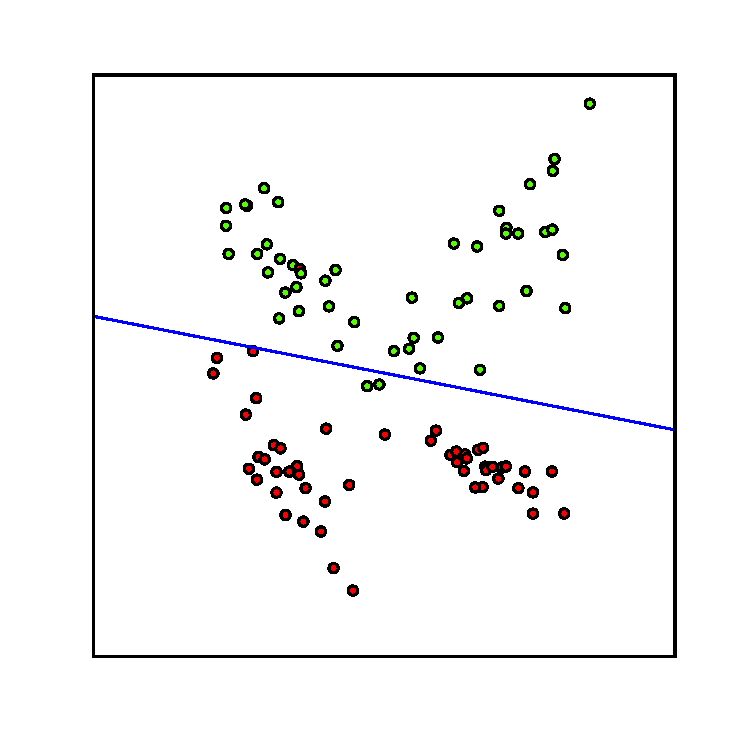
\includegraphics[width=1\linewidth]{logreg-pics/synthetic_line}\\

    \end{columns}
\end{frame}

\begin{frame}
    \frametitle{Example: Wisconsin Breast Cancer}
    \begin{columns}
        \column{.5\linewidth}
            \begin{itemize}
                \item Classify breast cancer samples in malign or benign.
                \item 699 Samples with 10 measurements each.
                \item We take only 3 measurements:
                    \begin{itemize}
                        \item Uniformity of Cell Size
                        \item Uniformity of Cell Shape
                        \item Single Epithelial Cell Size
                    \end{itemize}
                \item Training on 525, test on 175
                \item 97.1\% Accuracy
            \end{itemize}
        \column{.5\linewidth}
            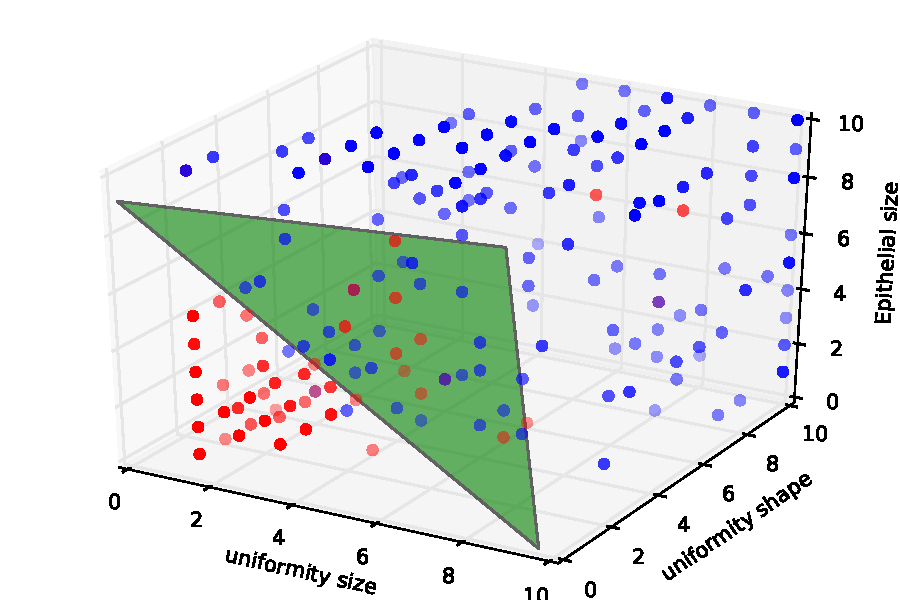
\includegraphics[width=1\linewidth]{logreg-pics/wisconsin_surface}
    \end{columns}

\end{frame}

\begin{frame}
    \frametitle{Mathematical Formulation I}
    \begin{columns}
        \column{.5\linewidth}
        \begin{itemize}
            \item For two classes $-1, +1$.
            \item Decision boundary given by hyperplane.
            \item Hyperplane defined by normal vector and offset:
                \begin{align*}
                    y = \text{sign}(\left<w, x\right> + b)
                \end{align*}
        \end{itemize}
        \column{.5\linewidth}
            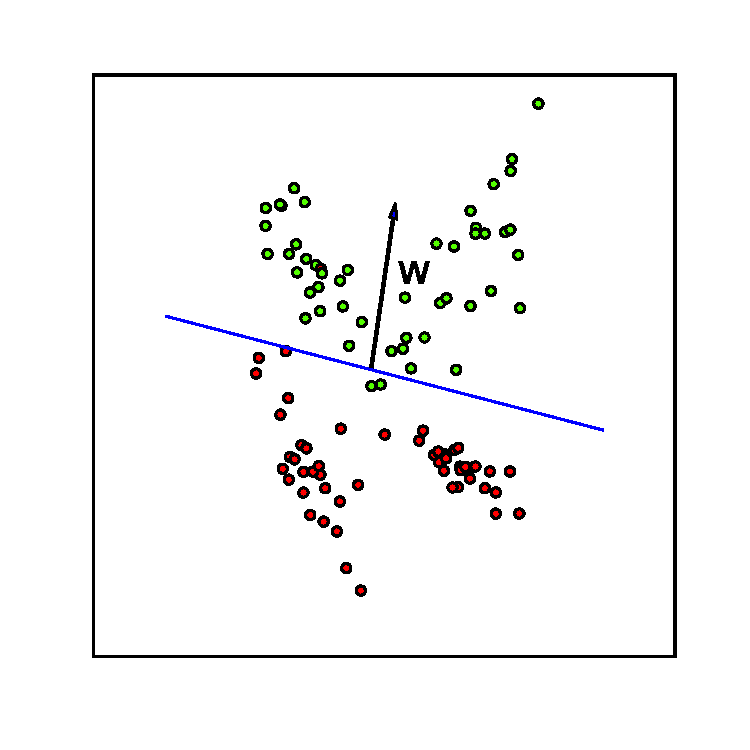
\includegraphics[width=1\linewidth]{logreg-pics/synthetic_line_w}\\

    \end{columns}
\end{frame}

\begin{frame}
    \frametitle{Mathematical Formulation II}
    \begin{itemize}
        \item Relation to regression:
            \begin{align}
                p(y=+1) = f(x) = \text{logistic}(\left<w, x\right> + b)
            \end{align}
        \item As probabilities are between $0$ and $1$, the logistic function
            squashes the regression result.
        \item $p(Y=+1 | x) > 0.5 \Leftrightarrow \left <w, x \right> + b > 0$
        \item Need to solve:
            \begin{align}
                \min_w \sum_{i=0}^n \log(p(Y=y_i | x_i))
            \end{align}
    \end{itemize}
\end{frame}


\begin{frame}
    \frametitle{Example: Classifying Insults}
    % coefficients are meaningful
\end{frame}

%\begin{frame}
    %\frametitle{Logistic Regression -- Interactive}
    %\begin{itemize}
        %\item some 2D blobs dataset
        %\item  Breast Cancer dataset
        %\item  http://archive.ics.uci.edu/ml/datasets/Breast+Cancer+Wisconsin+%28Diagnostic%29
    %\end{itemize}
%\end{frame}
